\subsection{完全格序空间中的带}

定义 4. --- 在完全格序空间 E 中，E 的线性子空间 B 称为一个带，如果它满足以下条件：1) 关系 \(x \in B\) 、\(y \in E\) 与 \(|y| \leqslant |x|\) 蕴涵 \(y \in B\) ；2) 对 B 的每个在 E 中有上界的非空子集 X，X 在 E 中的上确界 sup X 属于 B。

例. --- 在定义在集 A 上的实值函数所成的空间 \(R^{A}\) 中，在 A 的子集 M 的所有点上为零的函数所成的集是一个带。

\pandocbounded{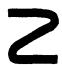
\includegraphics[keepaspectratio]{images/part001_20a85035.jpg}}

注. --- 在空间 \(R^{A}\) 中，A 上有界实值函数所成的子空间 \(\mathcal{B}(A)\) 满足定义 4 的条件 1)；此外，对 \(\mathcal{B}(A)\) 的每个在 \(\mathcal{B}(A)\) 中有上界的子集 X，X 的上包络属于 \(\mathcal{B}(A)\) 。然而，若 A 是无限集，\(\mathcal{B}(A)\) 的一个子集可能在 \(R^{A}\) 中有上界而在 \(\mathcal{B}(A)\) 中没有上界，在这种情形 \(\mathcal{B}(A)\) 不是 \(R^{A}\) 中的带。

由定义 4 立即得出：若 B 是 E 中的一个带，则对 B 的每个在 E 中有下界的非空子集 X，inf X 属于 B。E 中的每个带 B，赋以由 E 诱导的序向量空间结构，都是完全格序空间，且对 B 的每个在 B 中有上界的子集 \(X \subset B\) ，X 在 B 中的上确界与它在 E 中的上确界相同。

完全格序空间 E 中任意一族带的交仍是一个带。对每个子集 \(M \subset E\) ，存在包含 M 的最小带（因为 E 本身就是一个带）；这个带称为由 M 生成的带。

完全格序空间中带的性质以下述命题为基础：

命题 5. --- 设 E 是完全格序空间，A 是 E 的一个由元素 \(\geqslant 0\) 组成的非空子集，满足：1) \(A + A \subset A\) ；2) 关系 \(x \in A\) 、\(0 \leqslant y \leqslant x\) 蕴涵 \(y \in A\) 。设 M 是 A 的那些在 E 中有上界的子集在 E 中的上确界所成的集。在这些条件下，E 的每个元素 \(x \geqslant 0\) 都可写成 \(y + z\) 的形式，其中 \(y \in M\) 是元素 \(v \in A\) （满足 \(v \leqslant x\) 者）的上确界，而 z 是一个与 M 的每个元素互奇异的元素 \(\geqslant 0\) 。

无论如何 \(y \leqslant x\) ，因此问题归结为证明 z = x - y 与每个元素 \(t \in A\) 互奇异 (No. 1)，换句话说，\(u = \inf(z, t)\) 为零。由假设，\(u \in A\) 且 \(u \leqslant x - y\) ，于是 \(u + y \leqslant x\) ；对每个 \(v \in A\) ，若 \(v \leqslant x\) ，则由定义有 \(v \leqslant y\) ，于是 \(u + v \leqslant u + y \leqslant x\) ；由于由假设 \(u + v \in A\) ，由 y 的定义也有 \(u + v \leqslant y\) ；最后，由于 \(u + y\) 是元素 \(u + v\) （其中 \(v \in A\) 且 \(v \leqslant x\) ）在 E 中的上确界，我们有 \(u + y \leqslant y\) ，从而 \(u \leqslant 0\) ，证毕。

定理 1 (F. Riesz). --- 设 A 是完全格序空间 E 的一个子集。与 A 的每个元素互奇异的元素所成的集 A' 是一个带；由与 A' 的每个元素互奇异的元素组成的带 A'\,' 与由 A 生成的带相同，且 E 是诸带 A' 与 A'\,' 的序直和。

在第 1 小节中回顾的互奇异元素的性质以及带的定义立即表明 A' 是一个带，因而 A'\,' 也是一个带。由命题 5 及带的定义，E 的每个元素 \(x \geqslant 0\) 都可写成 \(x = y + z\) ，其中 \(y \in A'\) 且 \(z \in A''\) ，y 与 z 均 \(\geqslant 0\) ；由于 E 的每个元素都是两个 \(\geqslant 0\) 元素之差，我们有 \(E = A' + A''\) ；另一方面，由于 0 是唯一与自身互奇异的元素，我们有 \(A' \cap A'' = \{0\}\) ，这就证明 E 是 \(A'\) 与 \(A''\) 的直和；最后，由于在 \(A'\) 与 \(A''\) 中，E 的元素 \(\geqslant 0\) 的分量都 \(\geqslant 0\) ，E 是 \(A'\) 与 \(A''\) 的序直和 (No. 4, Prop. 4)。

剩下的是要证明 \(A''\) 与由 A 生成的带 B 相同。而 E 是 B 与由和 B 的所有元素互奇异的元素组成的带 \(B'\) 的直和；由于 \(A \subset B\) ，我们有 \(B' \subset A'\) ；另一方面 \(B \subset A''\) ，且 E 也是 \(A'\) 与 \(A''\) 的直和；因此必有 \(B = A''\) ，\(B' = A'\) 。

定理 1 与命题 5 使我们能够给出由 E 的一组元素生成的带的另一个定义：

命题 6. --- 设 E 是完全格序空间，M 是 E 的子集，B 是由 M 生成的带。设 \(M_{1}\) 是 E 中元素 \(\geqslant 0\) 所成的集，其中每个元素都 \(\leqslant\) 某个形如 \(\sum |x_{i}|\) 的元素，这里 \(x_{i} \in M\) ；

设 \(M_{2}\) 是 \(M_{1}\) 的那些有上界的子集的上确界所成的集；则集 \(M_{2}\) 与 B 中元素 \(\geqslant0\) 所成的集相同。

由带的定义，显然 \(M_{2} \subset B\) ；另一方面，若 \(B'\) 是由与 \(M_{1}\) 的每个元素互奇异的元素组成的带，则定理 1 表明 E 是 B 与 \(B'\) 的序直和。而命题 5 表明 E 的每个元素 \(\geqslant 0\) 是 \(M_{2}\) 的一个元素与 \(B'\) 的一个元素之和，由此即得本命题。

推论. --- 设 \(a\) 是完全格序空间 \(\mathbf{E}\) 的一个元素，\(\mathbf{B}_a\) 是由 \(a\) 生成的带，\(\mathbf{B}_a'\) 是与 \(a\) 互奇异的元素所成的带。对每个元素 \(x \geqslant 0\) （属于 \(\mathbf{E}\) ），\(x\) 在 \(\mathbf{B}_a\) 中的分量（相应于把 \(\mathbf{E}\) 分解为 \(\mathbf{B}_a\) 与 \(\mathbf{B}_a'\) 的序直和）等于 \(\sup_{n \in \mathbf{N}} \left( \inf(n|a|, x) \right)\) 。

这由把命题 6 应用于 \(\mathbf{M} = \{a\}\) 以及命题 5 得出。

注意，由 a 与 \(|a|\) 生成的带相同。若 a 与 b 是 E 的两个互奇异元素，且 A 与 B 分别是由 a 与 b 生成的带，则 A 的每个元素与 B 的每个元素互奇异；因为 b 属于由与 a 互奇异的元素组成的带 \(A'\) ，从而 \(B \subset A'\) ，且由定理 1，A 的每个元素与 \(A'\) 的每个元素互奇异。

